\documentclass[tikz,border=10pt]{standalone}

\usepackage{tikz}
\usetikzlibrary{shapes, arrows.meta, positioning, fit, calc, backgrounds, shadows}
\usepackage{amsmath, amssymb}
\usepackage{sourcesanspro}
\renewcommand{\familydefault}{\sfdefault}

\definecolor{cBlockFill}{RGB}{255, 235, 238} 
\definecolor{cBlockDraw}{RGB}{183, 28, 28}   
\definecolor{cBlockText}{RGB}{120, 10, 10} 

\definecolor{cLFFill}{RGB}{227, 242, 253}    
\definecolor{cLFDraw}{RGB}{21, 101, 192}     
\definecolor{cLFText}{RGB}{13, 71, 161}

\definecolor{cWFFill}{RGB}{232, 245, 233}    
\definecolor{cWFDraw}{RGB}{46, 125, 50}      
\definecolor{cWFText}{RGB}{27, 94, 32}

\tikzset{
    font=\sffamily,
    container/.style={
        rectangle, thick, rounded corners=6pt,
        drop shadow={opacity=0.15, shadow xshift=2pt, shadow yshift=-2pt},
        inner sep=0pt
    },
    contentBox/.style={
        anchor=north west,
        align=left,
        font=\small,
        inner xsep=10pt,
        inner ysep=10pt
    }
}

\newcommand{\labelWidth}{2.1cm}

\newcommand{\tabLabel}[1]{%
    \makebox[\labelWidth][l]{\textbf{#1}}%
}

\newcommand{\header}[2]{{\bfseries\Large\textcolor{#1}{#2}}\\[2pt]}
\newcommand{\tools}[2]{{\bfseries\scriptsize\textcolor{#1}{(#2)}}\\[8pt]}
\newcommand{\highlight}[2]{\textbf{\textcolor{#1}{#2}}}

\begin{document}

\begin{tikzpicture}[node distance=0cm]

	% =========================================================
	% 1. Blocking Synchronization
	% =========================================================

	\node [container, draw=cBlockDraw, fill=cBlockFill, minimum width=6cm] (blocking) {
		\begin{tikzpicture}
			\node [contentBox, text width=5.6cm] {
				\header{cBlockDraw}{Blocking}
				\tools{cBlockDraw}{Mutex, Spinlock, Condition Variable}

				\textit{``One stops, ALL stop."}\\[0.3cm]

				\tabLabel{Philosophy:} \highlight{cBlockText}{Pessimistic Control}\\[2pt]

				\tabLabel{Guarantee:} None.\\
				\quad Depends on OS scheduler.\\[2pt]

				\textbf{Risk:} Deadlock, Priority Inversion $\cdots$
			};
		\end{tikzpicture}
	};

	\node [anchor=south, font=\scriptsize\bfseries, color=cBlockDraw!60, yshift=-15pt]
	at (blocking.south) {Blocking Synchronization};

	% =========================================================
	% 2. Lock-Free
	% =========================================================

	\node [container, draw=cLFDraw, fill=cLFFill,
		minimum width=7cm, minimum height=9.0cm,
		right=1.5cm of blocking.north east, anchor=north west] (lockfree) {};

	\node [contentBox, text width=6.6cm] at (lockfree.north west) {
		\header{cLFDraw}{Lock-Free}
		\tools{cLFDraw}{CAS-based Algorithms, Lock-Free Data Structures}

		\textit{``System keeps moving."}\\[0.3cm]

		\tabLabel{Philosophy:} \highlight{cLFText}{Optimistic Control}\\[2pt]

		\tabLabel{Guarantee:} System-wide Progress.\\
		\quad At least one thread makes progress.\\[2pt]

		\textbf{Risk:} Starvation (Possible), Livelock $\cdots$
	};

	% =========================================================
	% 3. Wait-Free (Nested)
	% =========================================================

	\node [container, draw=cWFDraw, fill=cWFFill,
		minimum width=6.2cm, anchor=south, yshift=0.8cm]
	(waitfree) at (lockfree.south) {

		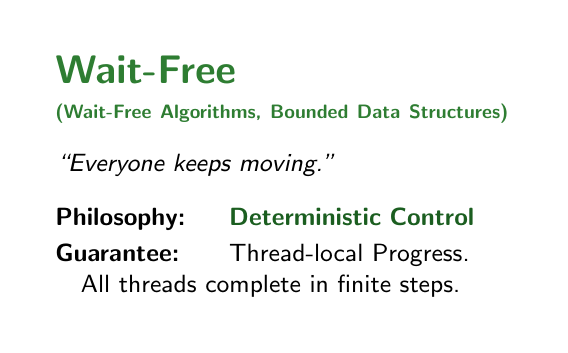
\begin{tikzpicture}
			\node [contentBox, text width=5.8cm] {
				\header{cWFDraw}{Wait-Free}
				\tools{cWFDraw}{Wait-Free Algorithms, Bounded Data Structures}

				\textit{``Everyone keeps moving."}\\[0.3cm]

				\tabLabel{Philosophy:} \highlight{cWFText}{Deterministic Control}\\[2pt]

				\tabLabel{Guarantee:} Thread-local Progress.\\
				\quad All threads complete in finite steps.
			};
		\end{tikzpicture}
	};

	\node [anchor=south, font=\scriptsize\bfseries, color=cLFDraw!60, yshift=-15pt]
	at (lockfree.south) {Non-Blocking Synchronization};

	% =========================================================
	% 4. Divider (Only)
	% =========================================================

	\draw [dashed, thick, color=black!20]
	($(blocking.east)!0.5!(lockfree.west) + (0, 4)$) --
	($(blocking.east)!0.5!(lockfree.west) + (0, -5)$);

\end{tikzpicture}

\end{document}
